\documentclass[10pt,letterpaper]{book}
\usepackage[utf8]{inputenc}
\usepackage[spanish]{babel}
\usepackage{amsmath}
\usepackage{amsfonts}
\usepackage{amssymb}
\usepackage{graphicx}
\usepackage{empheq}
\usepackage{svg}
\usepackage{hyperref}
\usepackage{hypcap}
\usepackage[spanish,onelanguage,linesnumbered,ruled,vlined]{algorithm2e}
\usepackage{titling}
\pretitle{%
  \begin{flushright}
  \vspace{-8.5cm}
%  \includegraphics[width=5cm,natwidth=472,natheight=531]{logo} \\[7cm]
  \includegraphics[width=5cm]{logo} \\[6cm]
  \end{flushright}
  \begin{center}
  \LARGE
}
\posttitle{\end{center}}
\usepackage[left=4cm,right=2.5cm,top=2cm,bottom=2cm,includehead,includefoot,headheight=15pt]{geometry}
\usepackage{setspace}
\setstretch{1}
\usepackage{fancyhdr}
\date{10 de Diciembre 2018}
\fancyhf{}
\renewcommand{\headrulewidth}{0pt} % optional
%\fancyhead[L]{\nouppercase{\leftmark} \hfill Section \nouppercase{\rightmark}}
\fancyhead[L]{Bases de Datos I - INF312}
\cfoot{\thepage}
\pagestyle{fancy}
\author{
Leonardo H. Añez Vladimirovna\\
\texttt{toborochi98@outlook.com}
\and
Mauricio Elian Delgadillo\\
\texttt{elianklk@gmail.com}
}
\title{
{\large \textbf{\textsc{INF312 - BASE DE DATOS I (SA)}}}\\\vspace{0.5cm}
{\large \textsc{Universidad Autónoma Gabriel René Moreno \\ \vspace{0.5cm} Facultad de Ingeniería en Ciencias de la Computación y\\ \vspace{0.4cm} Telecomunicaciones}} \vspace{0.5cm} 
\hrule\vspace{0.5cm}
{\LARGE \textsc{Base de Datos Hospitalaria}}
\vspace{0.5cm}
\hrule
}

\definecolor{dkgreen}{rgb}{0,0.6,0}
\definecolor{ltgray}{rgb}{0.5,0.5,0.5}

\usepackage{listings}
\lstset{%
  	backgroundcolor=\color{white},
  	basicstyle=\footnotesize\ttfamily,
  	breakatwhitespace=false,
  	breaklines=true,
  	captionpos=b,
  	commentstyle=\color{dkgreen},
  	deletekeywords={...},
  	escapeinside={\%*}{*)},
  	extendedchars=true,
  	frame=single,
  	keepspaces=true,
  	keywordstyle=\color{blue},
  	language=SQL,
  	morekeywords={*,modify,MODIFY,...},
  	numbers=left,
  	numbersep=15pt,
  	numberstyle=\tiny,
  	rulecolor=\color{ltgray},
  	showspaces=false,
  	showstringspaces=false, 
  	showtabs=false,
  	stepnumber=1,
  	tabsize=4,
  	title=\lstname
}

\begin{document}
\maketitle
El presente proyecto esta disponible en github, como codigo libre, junto con todo el material de este informe: \texttt{https://github.com/toborochi/Personal-Projects/tree/master/DB}
\vspace{-30cm}
\begin{center}

\includegraphics[width=2cm]{git}\\

\includegraphics[width=4cm]{DB312}
\end{center}
\pagebreak
\subsection*{Introducción}
El proyecto abordara el problema de registro de un sistema hospitalario a travez de las tres etapas de diseño: Conceptual, Lógico y Físico.
\subsection*{Planteamiento}
Esta base de Datos contendra datos demograficos del paciente, informacion de facturacion y seguros, asi como su historial medico. 
Permite realizar un seguimiento de los registros tanto de pacientes hospitalizados como ambulatorios. Se podra verificar la habitacion que ocupa actualmente un paciente hospitalizado, y los medicos podran identificar facilmente a sus pacientes, y determinar que enfermeras estan asignadas para ayudarlos en una determinada sala.

La base de datos requerirá muchos tipos diferentes de datos. Toda la información de contacto de los pacientes, como la dirección, el número de teléfono y el correo electrónico, será necesaria, así como toda la información de prescripción. Toda la información de la cita se registrará y guardará para que se extraiga cuando sea necesario. Si un paciente es un paciente interno, entonces se registrará la habitación en la que reside actualmente. También se almacenará información de facturación y seguro del paciente. También habrá datos almacenados para cada médico en el hospital, describiendo su especialidad, y supervisores. También habrá información sobre las enfermeras y la sala de las que están a cargo durante sus fechas y horarios de turnos especificados. Las enfermeras son responsables del cuidado de todos los pacientes que residen en sus salas y habitaciones designadas, y tendrán que informar a su supervisor de vez en cuando. \\
\linebreak
Para facilitar el proceso de elaboración del Diagrama, tendremos las siguientes asunciones:
\subsection*{Asunciones}
\begin{itemize}
\item Todos los pacientes deben tener una póliza de seguro para ser tratados en el hospital.
\item Un paciente puede someterse a muchos tratamientos en el hospital.
\item Un paciente puede o no recibir recetas de los médicos en el hospital.
\item Todas las enfermeras y médicos tienen supervisores.
\item Los pacientes recibirán cada costo de tratamiento bajo pagos individuales.
\item Los pacientes pueden realizar los pagos en cuotas múltiples.
\item Las enfermeras son asignadas a una sala durante su turno.
\item Los pacientes hospitalizados se registran en una habitación dentro de una sala apropiada.
\item Todos los médicos del hospital se especializan en un campo médico determinado.
\end{itemize}
\pagebreak
\section*{Diseño Conceptual}
\vspace{-5cm}
\begin{figure}[h!]
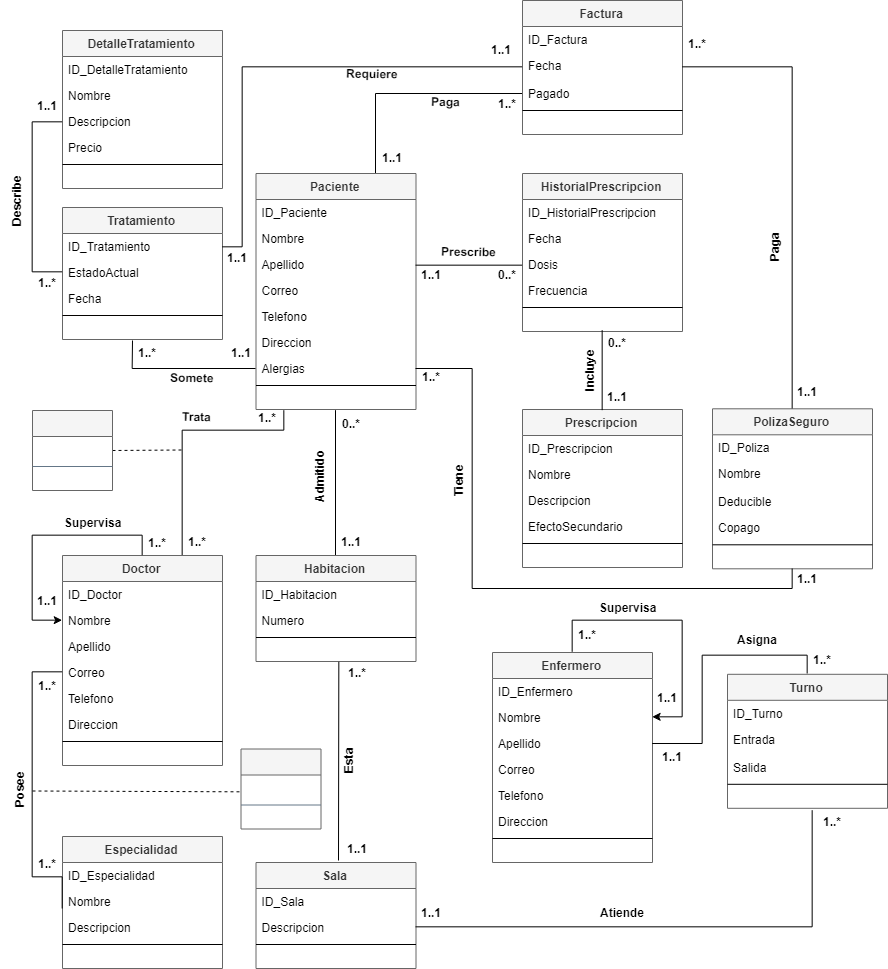
\includegraphics[width=15cm]{DConceptual} 
\caption{M.C. de la Base de Datos Hospitalaria}
\end{figure}
\pagebreak
\section*{Diseño Lógico}
Luego de realizar el Diseño Conceptual, procedemos a realizar el mapeo del diseño, con lo que tenemos la siguientes tablas:
\begin{center}
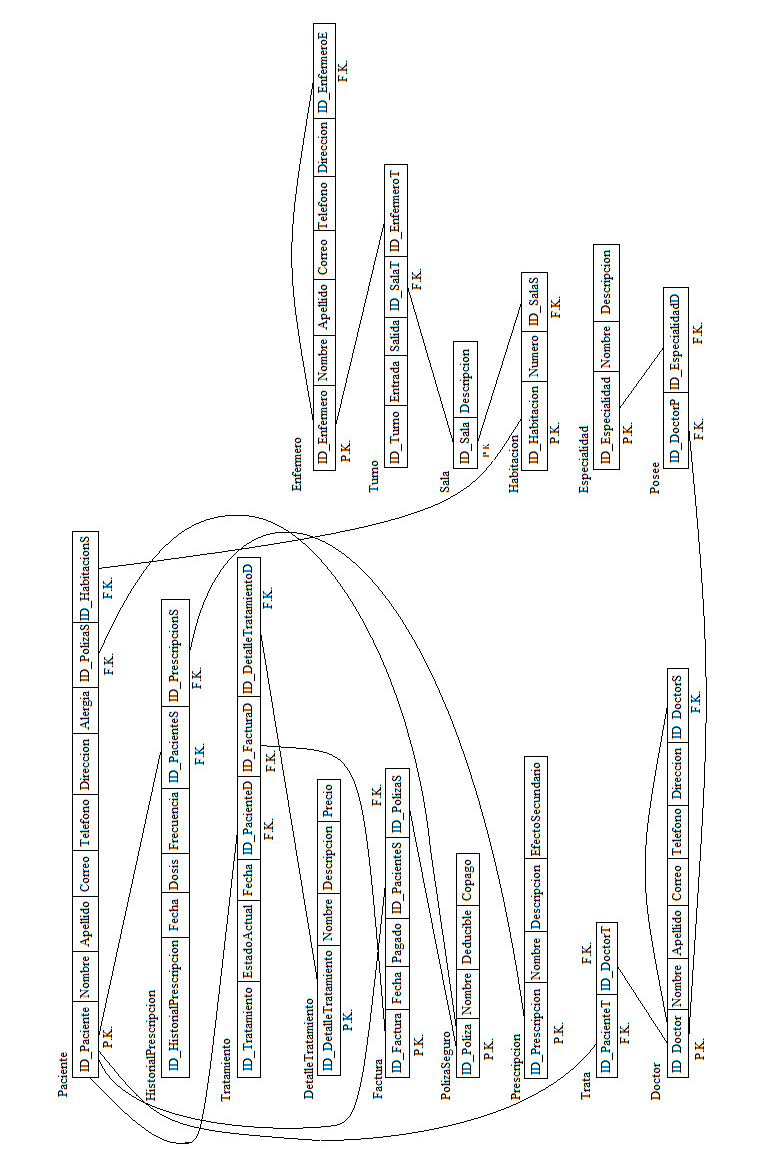
\includegraphics[width=13cm]{dd} 
\end{center}
\section*{Diseño Físico}
\subsubsection{Detalle Tratamiento}
\begin{lstlisting}[language=sql]
create table DetalleTratamiento(
	ID_DetalleTratamiento int not null,
	Nombre varchar(50) not null,
	Descripcion varchar(200) not null,
	Precio float not null,
	primary key(ID_DetalleTratamiento));
\end{lstlisting}
\subsubsection{Sala}
\begin{lstlisting}[language=sql]
create table Sala(
	ID_Sala int not null,
	Descripcion varchar(200) not null,
	primary key(ID_Sala));
\end{lstlisting}
\subsubsection{Habitacion}
\begin{lstlisting}[language=sql]
create table Habitacion(
	ID_Habitacion int not null,
	Numero int not null,
	SalaS int not null,
	primary key(ID_Habitacion),
	Foreign key(SalaS) references Sala(ID_Sala)
	On delete cascade
	On update cascade,);
\end{lstlisting}
\subsubsection{Poliza Seguro}
\begin{lstlisting}[language=sql]
create table PolizaSeguro(
	ID_Poliza int not null,
	Nombre varchar(50) not null,
	Deducible float not null,
	Copago float not null,
	primary key(ID_Poliza),);
\end{lstlisting}
\subsubsection{Especialidad}
\begin{lstlisting}[language=sql]
create table Especialidad(
	ID_Especialidad int not null,
	Nombre varchar(50) not null,
	Descripcion varchar(200) not null,
	primary key(ID_Especialidad),);
\end{lstlisting}
\subsubsection{Paciente}
\begin{lstlisting}[language=sql]
create table Paciente(
	ID_Paciente int not null,
	Nombre varchar(50) not null,
	Apellido varchar(50) not null,
	Correo varchar(50),
	Telefono int ,
	Direccion varchar(50) not null,
	Alergia varchar(50) not null,
	ID_PolizaS int not null,
	ID_HabitacionS int not null
	primary key(ID_Paciente),
	Foreign key(ID_PolizaS) references PolizaSeguro(ID_Poliza)
	On delete cascade
	On update cascade,
	Foreign key(ID_HabitacionS) references Habitacion(ID_Habitacion)
	On delete cascade
	On update cascade);
\end{lstlisting}
\subsubsection{Factura}
\begin{lstlisting}[language=sql]
create table Factura(
	ID_Factura int not null,
	Fecha date not null,
	Pagado float not null,
	ID_PacienteF int not null,
	ID_PolizaF int not null,
	Primary key(ID_Factura),
	foreign key(ID_PacienteF) references Paciente(ID_Paciente)
	on delete no action
	On update no action,
	foreign key(ID_PolizaF) references PolizaSeguro(ID_Poliza)
	On delete no action
	On update no action);
\end{lstlisting}
\subsubsection{Prescripcion}
\begin{lstlisting}[language=sql]
create table Prescripcion(
	ID_Prescripcion int not null,
	Nombre varchar(50) not null,
	Descripcion varchar(200) not null,
	EfectoSegundario varchar(200) not null,
	primary key(ID_Prescripcion),);
\end{lstlisting}
\pagebreak
\subsubsection{Tratamiento}
\begin{lstlisting}[language=sql]
create table Tratamiento(
	ID_Tratamiento int not null,
	EstadoActual varchar(50) not null,
	Fecha varchar(8) not null,
	ID_PacienteD int not null,
	ID_FacturaD int not null,
	ID_DetalleTratamientoD int not null,
	primary key(ID_Tratamiento),
	Foreign key(ID_PacienteD) references Paciente(ID_Paciente)
	On delete cascade
	On update cascade,
	Foreign key(ID_FacturaD) references Factura(ID_Factura)
	On delete cascade
	On update cascade,
	Foreign key(ID_DetalleTratamientoD) references DetalleTratamiento(ID_DetalleTratamiento)
	On delete cascade
	On update cascade);
\end{lstlisting}
\subsubsection{Enfermero}
\begin{lstlisting}[language=sql]
create table Enfermero(
	ID_Enfermero int not null,
	Nombre varchar(50) not null,
	Apellido varchar(50) not null,
	Correo varchar(50),
	Telefono int ,
	Direccion varchar(50) not null,
	ID_EnfermeroS int null, 
	primary key(ID_Enfermero),
);

alter table Enfermero
add foreign key (ID_EnfermeroS) references Enfermero(ID_Enfermero)
on update no action
on delete no action;
\end{lstlisting}
\subsubsection{Trata}
\begin{lstlisting}[language=sql]
create table Trata(
	ID_DoctorT int not null,
	ID_PacienteT int not null,
	primary key (ID_DoctorT,ID_PacienteT),
	Foreign key (ID_DoctorT) references Doctor(ID_Doctor)
	on update no action
	on delete no action,
	Foreign key (ID_PacienteT) references Paciente(ID_Paciente)
	on update no action
	on delete no action);
\end{lstlisting}
\subsubsection{Doctor}
\begin{lstlisting}[language=sql]
create table Doctor(
	ID_Doctor int not null,
	Nombre varchar(50) not null,
	Apellido varchar(50) not null,
	Correo varchar(50),
	Telefono int ,
	Direccion varchar(50) not null,
	ID_DoctorS int ,
	primary key(ID_Doctor),
);


alter table Doctor
add foreign key (ID_DoctorS) references Doctor(ID_Doctor)
on update no action
on delete no action;
\end{lstlisting}
\subsubsection{Posee}
\begin{lstlisting}[language=sql]
create table Posee(
	ID_DoctorP int not null,
	ID_EspecialidadP int not null,
	primary key (ID_DoctorP,ID_EspecialidadP),
	Foreign key (ID_DoctorP) references Doctor(ID_Doctor)
	on update no action
	on delete no action,
	Foreign key (ID_EspecialidadP) references Especialidad(ID_Especialidad)
	on update no action
	on delete no action);
\end{lstlisting}
\subsubsection{Turno}
\begin{lstlisting}[language=sql]
create table Turno(
	ID_Turno int not null,
	Entrada date not null,
	Salida varchar(8) not null,
	ID_SalaT int not null,
	ID_EnfermeroT int null,
	primary key(ID_Turno),
	Foreign key(ID_SalaT) references Sala(ID_Sala)
	On delete cascade
	On update cascade,
	Foreign key(ID_EnfermeroT) references Enfermero(ID_Enfermero)
	On delete cascade
	On update cascade);
\end{lstlisting}
\pagebreak
\subsubsection{Historial Prescripcion}
\begin{lstlisting}[language=sql]
create table HistorialPrescripcion(
	ID_HistorialPrescripcion int not null,
	Fecha date not null,
	Dosis int not null,
	Frecuencia int not null,
	ID_PacienteH int not null,
	ID_PrescripcionH int not null,
	primary key(ID_HistorialPrescripcion),
	Foreign key(ID_PacienteH) references Paciente(ID_Paciente)
	On delete cascade
	On update cascade,
	Foreign key(ID_PrescripcionH) references Prescripcion(ID_Prescripcion)
	On delete cascade
	On update cascade);
\end{lstlisting}

\end{document}